\documentclass[final]{beamer}

\mode<presentation>
{
  \definecolor{berkeleyblue}{HTML}{003A70}
  \definecolor{berkeleygold}{HTML}{F2A900}
%http://www.berkeley.edu/brand/img/downloads/UCB%20Brand%20Guidelines_FINAL_small.pdf
  \usetheme{I6dv}      % or try Darmstadt, Madrid, Warsaw, ...
  %\usecolortheme{dove} % or try albatross, beaver, crane, ...
  \setbeamercolor{structure}{fg=berkeleygold,bg=berkeleyblue}
  \setbeamercolor{palette primary}{fg=berkeleyblue,bg=berkeleygold} % changed this
  \setbeamercolor{palette secondary}{bg=berkeleyblue,fg=white} % changed this
  \setbeamercolor{palette tertiary}{bg=berkeleyblue,fg=white} % changed this
\setbeamercolor{bibliography item}{bg=white,fg=black}
\setbeamercolor{bibliography entry author}{bg=white,fg=black}
\setbeamercolor{bibliography entry journal}{bg=white,fg=black}
\setbeamercolor{bibliography entry note}{bg=white,fg=black}
  \usefonttheme{structurebold}  % or try serif, structurebold, ...
  \useinnertheme{circles}
  \setbeamertemplate{navigation symbols}{}
  \setbeamertemplate{footline}[title]{}
  \setbeamertemplate{footline}[author]{}
  \usebackgroundtemplate{
%  \tikz[overlay,remember picture] %Can insert a Berkeley watermark
%  \node[opacity=1, at=(current page.south west),anchor=south west, inner sep=2pt] {
%    \includegraphics[height=.5in,width=.5in]{img/ucseal_540_139.eps}};
}
}
\usepackage[sorting=none]{biblatex} 
  \usepackage{ragged2e}
  \usepackage{type1cm}
  \usepackage{calc} 
  \usepackage{times}
  \usepackage{amsmath,amsthm, amssymb, latexsym}
%  \boldmath
  \usepackage[english]{babel}
  \usepackage[latin1]{inputenc}
  \usepackage[orientation=landscape,size=a0,scale=1.4,debug]{beamerposter}
  \graphicspath{{img/}}
  %\title[Fancy Posters]{Making Really Fancy Posters with \LaTeX}
  %\author[Dreuw \& Deselaers]{Philippe Dreuw and Thomas Deselaers}
  %\institute[University of California, Berkeley]{Department of Nuclear Engineering}
  \newcommand{\footlinetext}{}

\bibliography{poster}
\setbeamertemplate{bibliography item}[text]

\title[Short Title]{Long, Appropriately Descriptive Title}
\author[A.B. Authorson et al.]{Author B. Authorson, Author C. McAuthor, Author D. Smith, Author E. Jones}
  \institute[UC Berkeley]{Department of Nuclear Engineering, University of California, Berkeley}
  \date{February 31, 1900}

\begin{document}
	\begin{frame}{}
%    \maketitle

%%%%%%%%%%%%%%
% FIRST COLUMN
%%%%%%%%%%%%%%

  		\begin{columns}[t]
    		\begin{column}{.3\linewidth}
    			\vfill
    			\begin{block}{\large Title}
      			\begin{itemize}
			\item{Bullet}
			\item{Bullet}
			\item{Bullet}
			\item{Bullet}
			\item{Bullet with cited information \cite{wiki:comp}}
			\end{itemize}
    			\end{block}
    	\vfill
    			\begin{block}{\large Computers}
			\begin{figure}[h!]
			\centering
	      		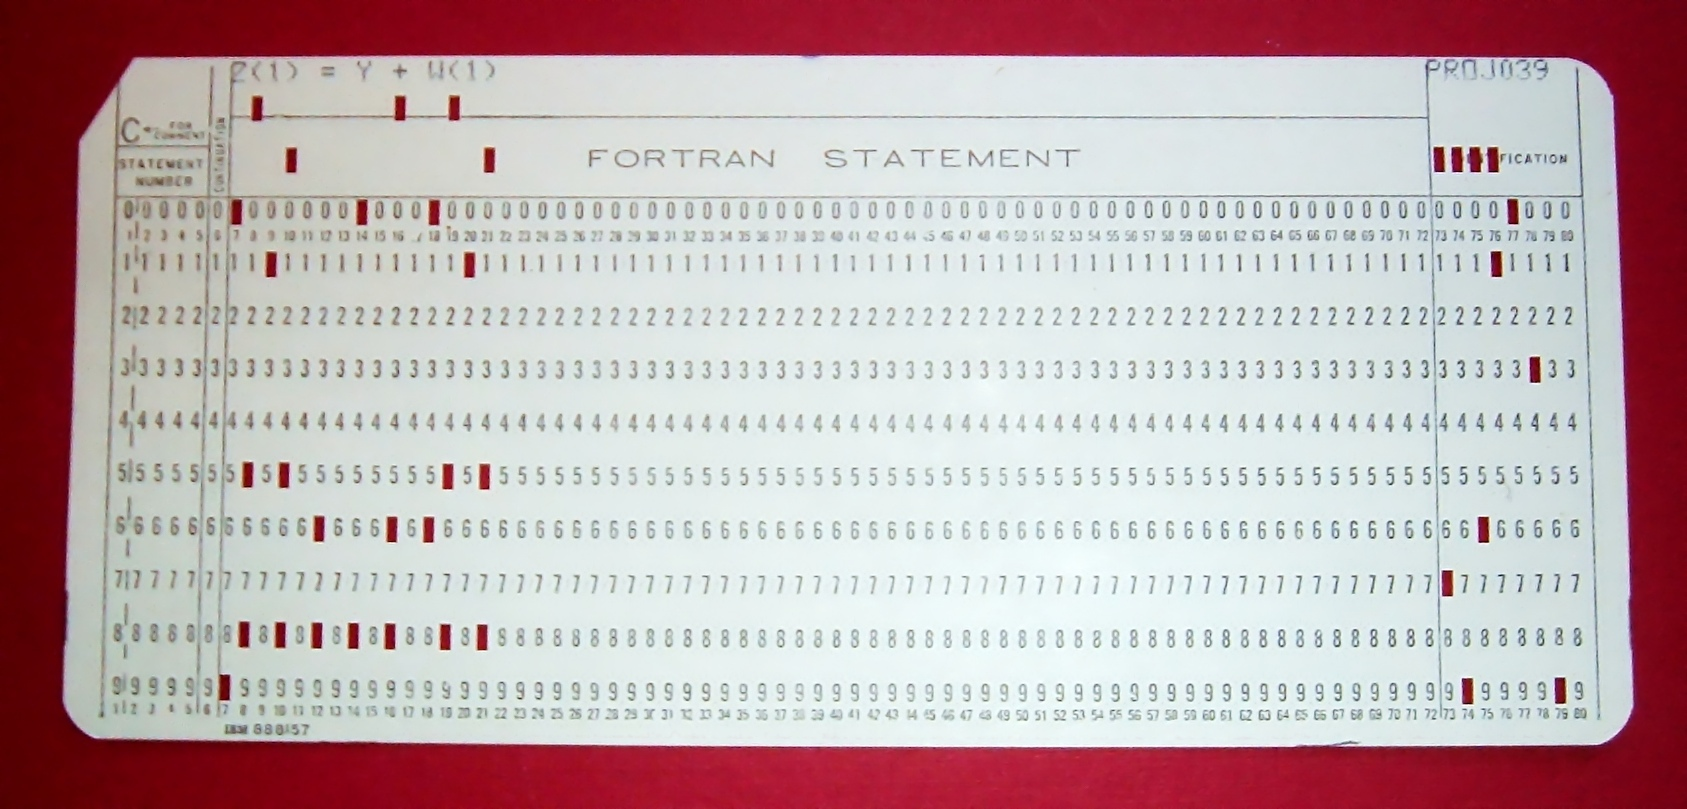
\includegraphics[width=10in]{FortranCardPROJ039.jpg}
			\newline
			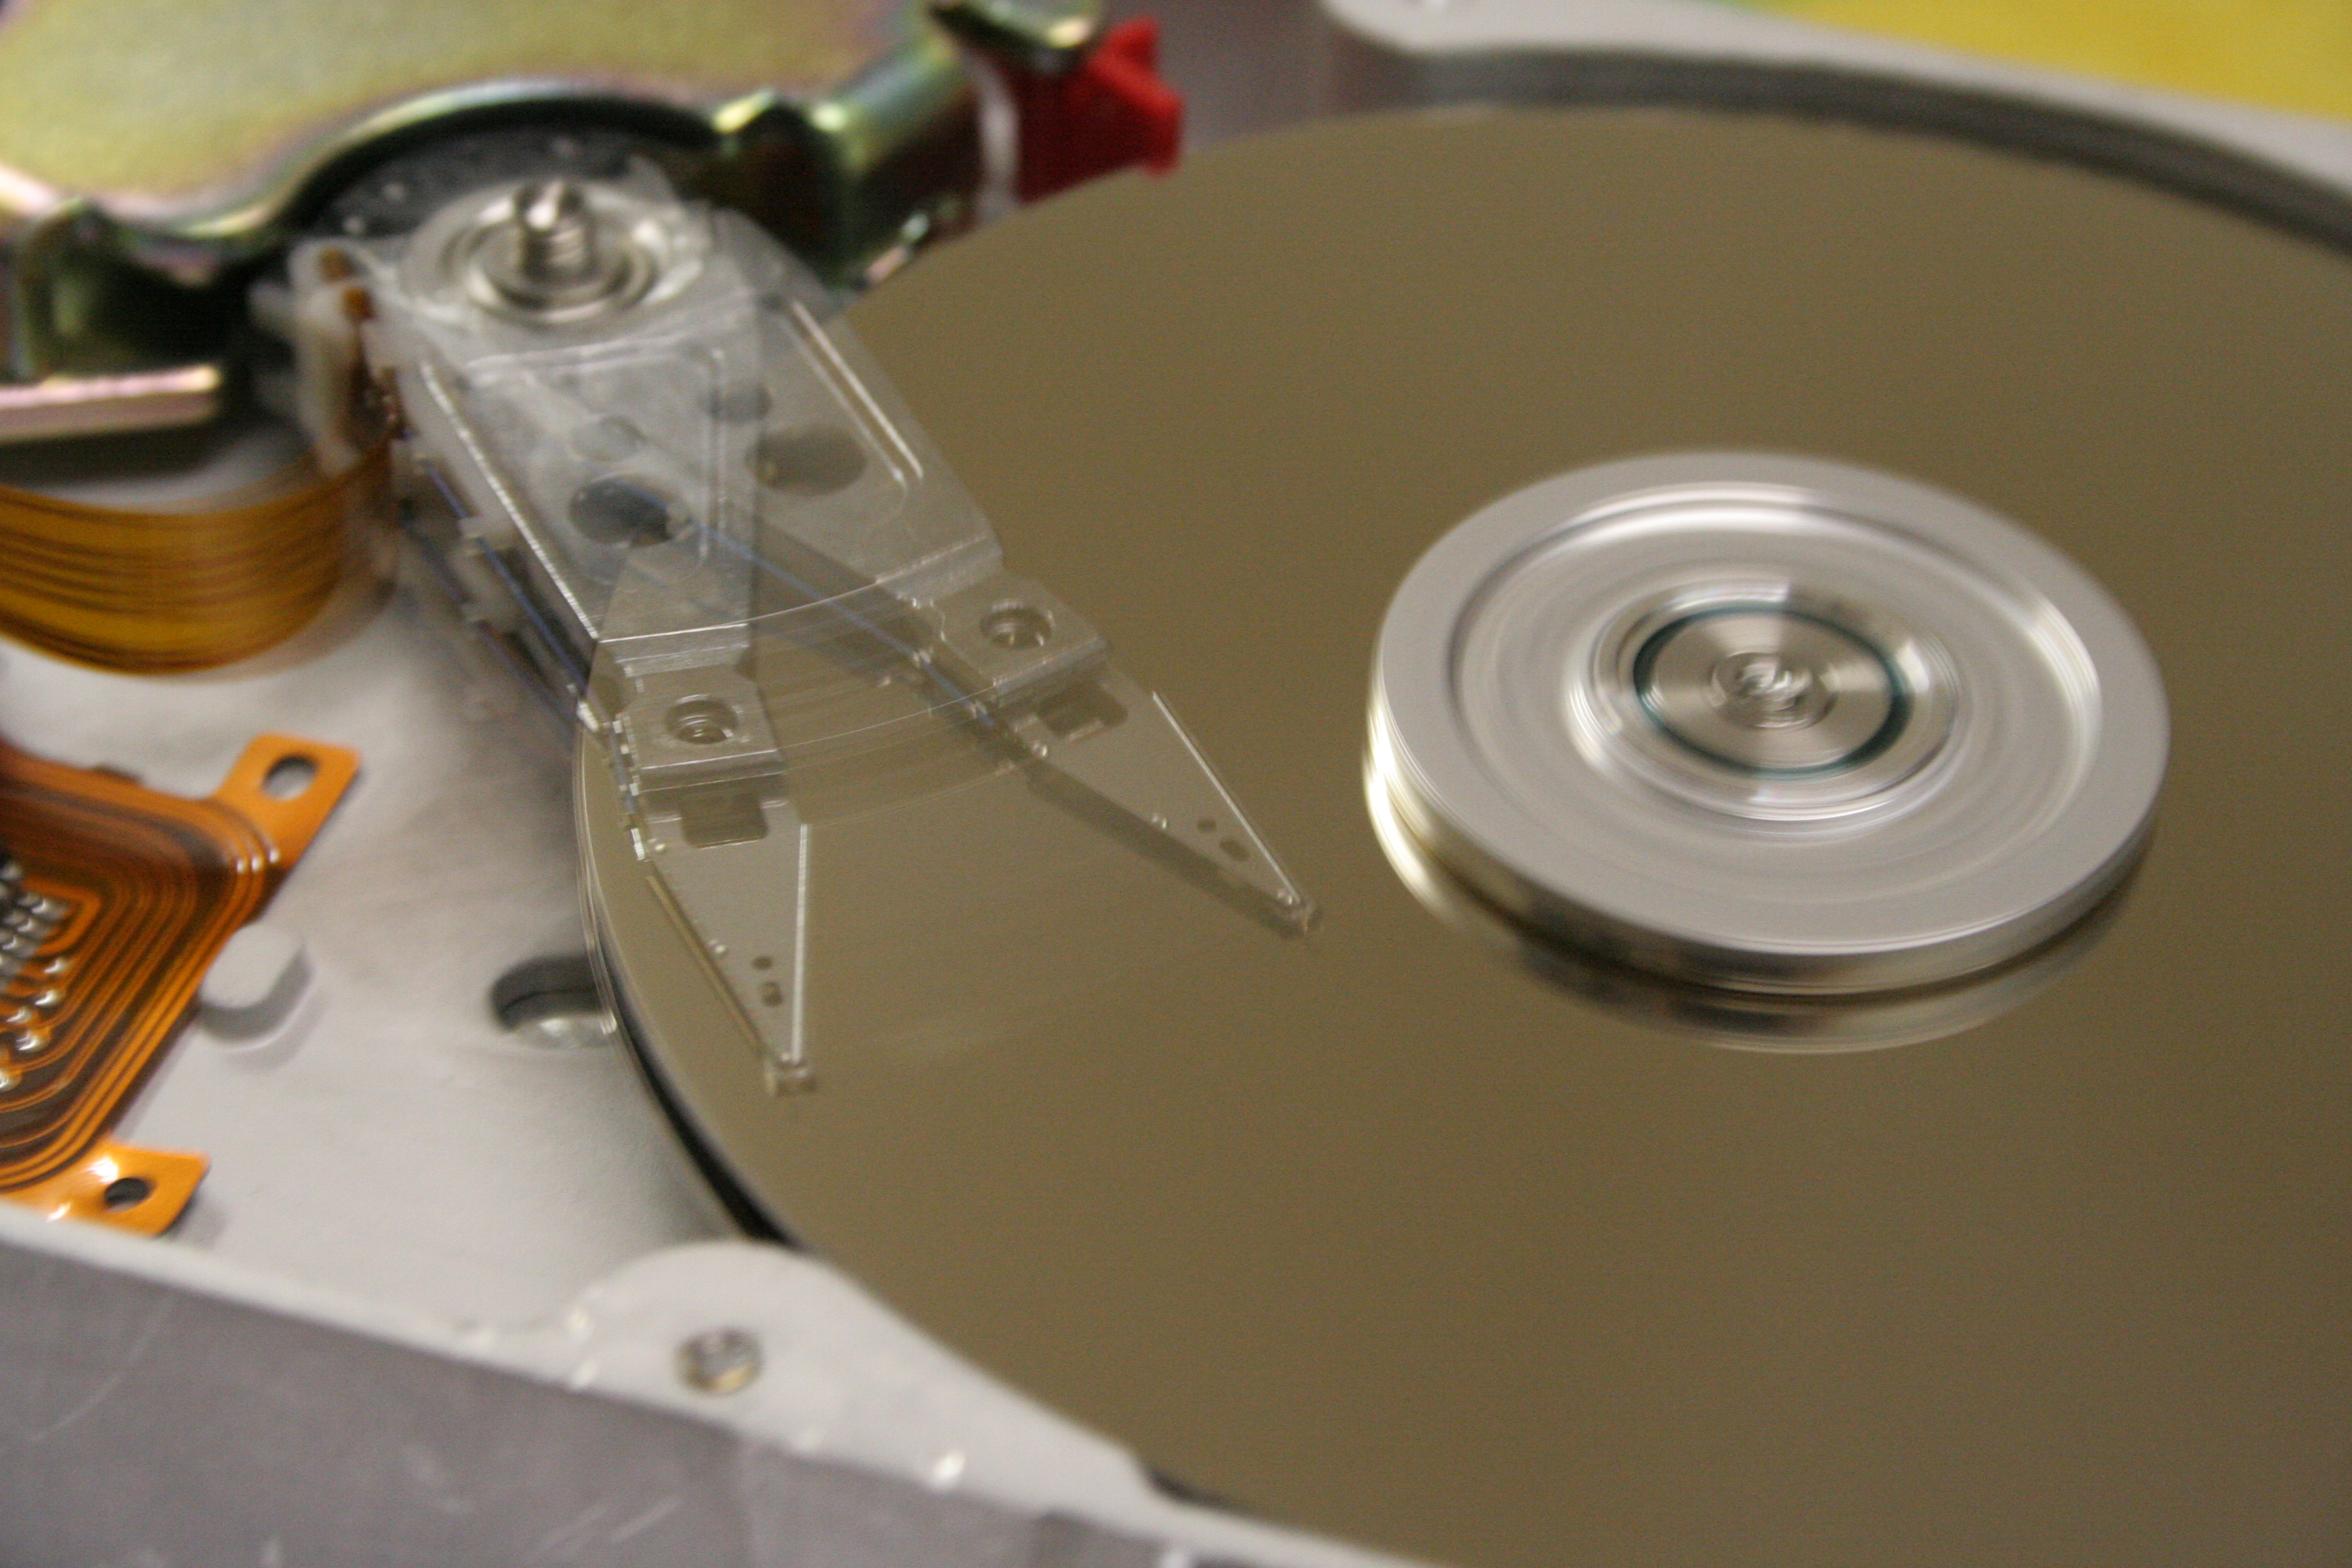
\includegraphics[width=10in]{HDDspin.JPG}
			\caption{Top: A punch card. Bottom: A hard disk drive \cite{wiki:comp}.}
			\end{figure}
			\begin{itemize}
			\item{The punch card contrains one line from a FORTRAN program \cite{wiki:comp}}
			\item{Hard disk drives are more commonly used these days}
			\end{itemize}
    			\end{block}
    	\vfill
        	\begin{block}{\large Force, Mass, and Acceleration}
		\begin{itemize}
		\item{These quantities are related as:}
			\begin{equation*}
			F = ma
			\end{equation*}
		\item{physics is cool}
		\item{but sometimes it can be confusing}
		\item{especially when you involve relativity}
		\end{itemize}
        	\end{block}
    	\end{column}

%%%%%%%%%%%%%%%
% SECOND COLUMN
%%%%%%%%%%%%%%%

      	\begin{column}{.3\linewidth}
            \begin{block}{Another Title}
	\begin{itemize}
	\item{Bullet}
		\begin{itemize}
		\item{Sub-bullet}
		\end{itemize}
	\item{More equations:}
		\begin{equation*}
		a^2 + b^2 = c^2
		\end{equation*}
	\item{Here comes the complicated stuff:}
		\begin{equation*}
		\begin{aligned}
		E &= mc^2 \\
		i^2 &= -1
		\end{aligned}
		\end{equation*}
	\item{Math is fun too}
	\item{Triangles are a great shape}
	\item{Here's the second law of thermodynamics:}
		\begin{equation*} 
		dS \geq 0
		\end{equation*}
	\item{Energy and heat dissipate over time}
	\end{itemize}
            \end{block}
		\vfill
        	\begin{block}{\large Bullets with no Equations}
          		\begin{itemize}
			\item{Less exciting, but still information}
			\item{Bullet}
			\item{Bullet}
			\item{Bullet}
			\end{itemize}
        	\end{block}
			\vfill
		\begin{block}{\large Results}
\begin{columns}
	\column{0.3\linewidth}
	\begin{figure}[h!]
	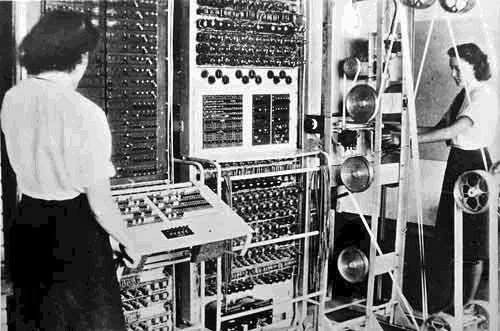
\includegraphics[width=6in]{Colossus.jpg}
	\caption{\footnotesize Colossus, a cipher-breaking machine \cite{wiki:comp}.}
	\end{figure}
	\column{0.7\linewidth}
	\begin{table}[h]
	\begin{tabular}{ll}
	\multicolumn{2}{c}{Table Title} \\ \hline
	Code 1, Ver. 1 & $val \pm \sigma$ \\
	Code 1, Ver. 2 & $val \pm \sigma$ \\
	Code 2, Ver. 1 & $val \pm \sigma$ \\
	Code 2, Ver. 2 & $val \pm \sigma$
	\end{tabular}
	\end{table}
	\begin{table}[h]
	\begin{tabular}{ll}
	\multicolumn{2}{c}{Runtimes} \\ \hline
	Code 1, Ver. 1 & slow \\
	Code 1, Ver. 2 & fast \\
	Code 2, Ver. 1 & slow \\
	Code 2, Ver. 2 & slow 
	\end{tabular}
	\end{table}
\end{columns}
	\begin{itemize}
	\item Code 1 is faster than Code 2
		\begin{itemize}
		\item But is it sufficiently accurate?
		\end{itemize}
	\item Make sure to analyze results carefully!
	\end{itemize}
		\end{block}
	\vfill
      \end{column}

%%%%%%%%%%%%%%
% THIRD COLUMN
%%%%%%%%%%%%%%

      \begin{column}{.3\linewidth}
		\begin{block}{Results - Another Computer}
\begin{columns}
	\column{0.4\linewidth}
	\begin{figure}[h!]
	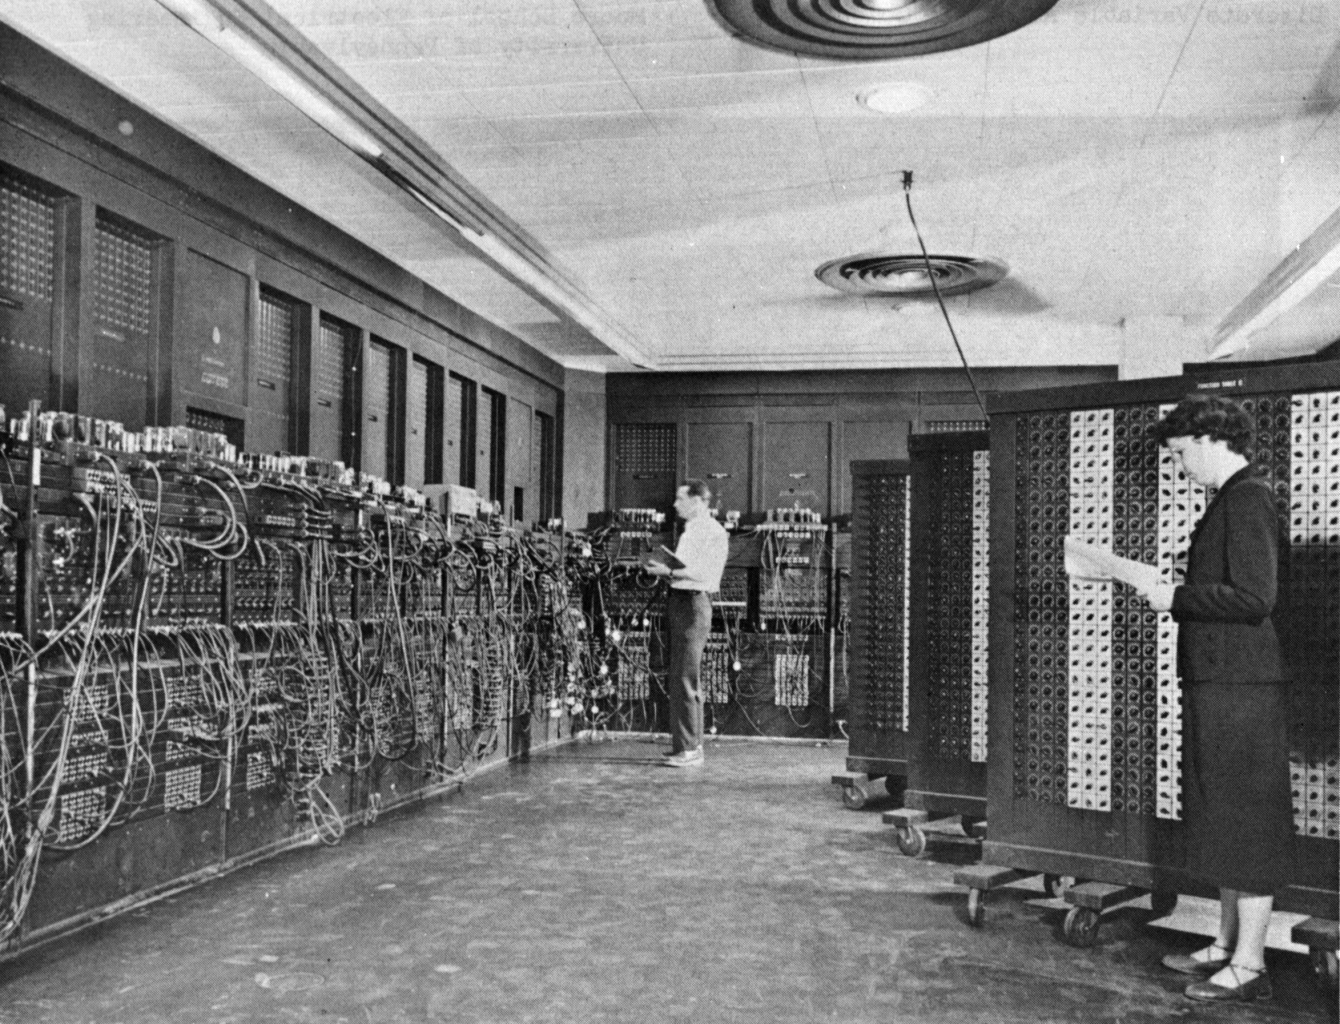
\includegraphics[width=5.5in]{Eniac.jpg}
	\caption{ENIAC, the first Turing-complete machine \cite{wiki:comp}.}
	\end{figure}
	\column{0.6\linewidth}
	\begin{itemize}
	\item{First electronic programmable computer built in the US}
	\item{Faster and more flexible than Colossus \cite{wiki:comp}}
	\end{itemize}
	\begin{table}[h]
	\begin{tabular}{ll}
	\multicolumn{2}{c}{ENIAC Results} \\ \hline
	Code 1, Ver. 1 & $val \pm \sigma$ \\
	Code 1, Ver. 2 & $val \pm \sigma$ \\
	Code 2, Ver. 1 & $val \pm \sigma$ \\
	Code 2, Ver. 2 & $val \pm \sigma$
	\end{tabular}
	\end{table}
	\begin{table}[h]
	\begin{tabular}{ll}
	\multicolumn{2}{c}{ENIAC Runtimes} \\ \hline
	Code 1, Ver. 1 & fast \\
	Code 1, Ver. 2 & very fast \\
	Code 2, Ver. 1 & fast \\
	Code 2, Ver. 2 & fast 
	\end{tabular}
	\end{table}
\end{columns}
		\end{block}
			\vfill
        	\begin{block}{\large Future Work}
          		\begin{itemize}
          		\item Build better computers
			\item Maybe vector machines?
          		\item Have some fun!
          		\end{itemize}
        	\end{block}
			\vfill
        	\begin{block}{\large References}
			\printbibliography
        	\end{block}
			\vfill
        	\begin{block}{\large Acknowledgements}
		\justifying
This material is based upon work supported under a Fungineering Fellowship. This work was partially supported by the Department of Excellence under Award Number(s) 3: The Good Work Association.
        	\end{block}
      \end{column}
    \end{columns}
  \end{frame}
\end{document}

%    			\begin{block}{\large Fontsizes}
%      				\centering
%      				{\tiny tiny}\par
%      				{\scriptsize scriptsize}\par
%      				{\footnotesize footnotesize}\par
%      				{\normalsize normalsize}\par
%      				{\large large}\par
%      				{\Large Large}\par
%      				{\LARGE LARGE}\par
%      				{\veryHuge VeryHuge}\par
%      				{\VeryHuge VeryHuge}\par
%      				{\VERYHuge VERYHuge}\par
%    			\end{block}

%%%%%%%%%%%%%%%%%%%%%%%%%%%%%%%%%%%%%%%%%%%%%%%%%%%%%%%%%%%%%%%%%%%%%%%%%%%%%%%%%%%%%%%%%%%%%%%%%%%%
%%% Local Variables: 
%%% mode: latex
%%% TeX-PDF-mode: t
